\documentclass{sig-alternate-05-2015}

\usepackage{mathtools,MnSymbol}
\usepackage{graphicx}
\usepackage{caption}
\usepackage{subcaption}
\usepackage{url}
\usepackage{cite}
%\usepackage{amsthm}


\allowdisplaybreaks



%\addtolength{\textwidth}{1in}
%\addtolength{\oddsidemargin}{-0.6in}
%\addtolength{\evensidemargin}{-0.6in}
\addtolength{\textheight}{0.4cm}
\addtolength{\topmargin}{-0.2cm}
%\leftmargini 2.9ex


\begin{document}



%\theoremstyle{definition}
\newtheorem{example}{Example}[section]


\newcommand{\ident}[1]{\texttt{#1}}
\newcommand{\tuple}[1]{\langle #1 \rangle}


\newcommand{\qqquad}{\qquad\qquad}
\newcommand{\qqqquad}{\qqquad\qqquad}
\newcommand{\qqqqquad}{\qqqquad\qqqquad}


\newcommand{\cA}{\mathcal{A}}



\newcommand{\Ev}{Ev}
\newcommand{\oR}{\overline{R}}

\newcommand{\facc}[2]{#1.\text{\small{#2}}}
\newcommand{\syms}[1]{{#1}^{\sigma}}
\newcommand{\symv}[1]{\text{\texttt{#1}}}

\newcommand{\precs}[1]{\phi_{#1}}
\newcommand{\heurs}[1]{\gamma_{#1}}

\newcommand{\slice}[2]{\text{Slice}_{#2}(#1)}


% Copyright
%\setcopyright{acmcopyright}
%\setcopyright{acmlicensed}
%\setcopyright{rightsretained}
%\setcopyright{usgov}
%\setcopyright{usgovmixed}
%\setcopyright{cagov}
%\setcopyright{cagovmixed}


\title{Jumping the ORDER BY barrier in large-scale pattern matching}

\begin{comment}
\numberofauthors{5} 
\author{
\alignauthorb
Daniel Lupei\\
   \affaddr{EPFL}\\
   \email{daniel.lupei@epfl.ch}
\alignauthor
Mike Barnett\\
   \affaddr{MSR, Redmond}\\
   \email{mbarnett@microsoft.com}
\alignauthor
Saeed Maleki\\
   \affaddr{MSR, Redmond}\\
   \email{saemal@microsoft.com}
\and
\alignauthor
Madan Musuvathi\\
   \affaddr{MSR, Redmond}\\
   \email{madanm@microsoft.com}
\alignauthor 
Todd Mytkowicz\\
       \affaddr{MSR, Redmond}\\
       \email{toddm@microsoft.com}
}
\end{comment}

\maketitle
\begin{abstract}
Event-series pattern matching is a major component of large-scale data 
analytics pipelines enabling a wide range of system diagnostics tasks.  
%While existing solutions focus on the online scenario and expect 
%their data to be (mostly) sorted on time, this is not the case in many 
%situations where batch processing is preferable due to the large volume of data 
%and where the physical data layout has to meet wider system requirements. 
A precursor to pattern matching is an expensive ``shuffle the world'' stage
wherein data are ordered by time and shuffled across the network.  Because many
existing systems treat the pattern matching engine as a black box, they are
unable to optimizing the entire data analytics pipeline, and in particular, this
costly shuffle.

This paper demonstrates how to optimize such queries. We first translate an
expressive class of regular-expression like patterns to relational queries such
that they can benefit from decades of progress in relational optimizers, and
then we introduce the technique of {\em abstract pattern matching}, a linear
time preprocessing step which, adapting ideas from symbolic execution and
abstract interpretation, discards events from the input guaranteed not to appear
in successful matches.  Abstract pattern matching first computes a conservative
representation of the output-relevant domain of every transition in a pattern
based on the (unary) predicates of that transition.  It then further refines
these domains based on the structure of the pattern (i.e., paths through the
pattern) as well as any of the pattern's join predicates across transitions.
The outcome is an {\em abstract filter} that when applied to the original stream
excludes events that are guaranteed not to participate in a match.

We implemented and applied {\em abstract pattern matching} in COSMOS/Scope to 
an industrial benchmark where we obtained up to 3 orders of magnitude reduction 
in shuffled data and 1.23x average speedup in total processing time.
% and 1.09x average speedup in end-to-end latency
\end{abstract}

\section{Introduction}

%(Motivation)

Event-series pattern matching has become essential to many data processing tasks
as it enables complex behavioral, anomaly, and causality analyses, in varied
domains ranging from network diagnostics and security breach detection, to
algorithmic trading or click-path optimization.  This trend prompted the
addition of pattern matching constructs to many batch and stream processing
engines such as Esper's Event Processing Language (EPL)~\cite{esper_epl},
Oracle's \texttt{MATCH\_RECOGNIZE}~\cite{oracle_mr} or TerraData's 
\texttt{nPath} operator~\cite{aster_npath}.
% or Splunk's Search Processing Language~\cite{Carasso:2012}.

These languages let programmers specify patterns as a series of transitions,
wherein a transition 
is triggered if the current event satisfies a guard defined in terms of both 
unary\allowbreak (selection) predicates as well as join conditions on 
priorly matched 
events. 
For example, a programmer might mine
influential reviews within the click-stream of an e-commerce website consisting
of events of type ``Search''(S), ``Read review''(R) and ``Purchase''(P) by
defining the pattern SR*P where each transition is joined on a userid (i.e.,
to make sure that all events in a match are correlated by the id of the user 
that performed them).

%(Challenges)
Pattern matching is usually only one of many stages in a data processing
pipeline.  As most of these stages are defined using relational queries (for 
eg., to enrich ingested data), the presence of pattern matching operators raises
considerable challenges in terms of deriving optimum execution plans.  Pattern
matching operators do not enjoy the same wealth of rewriting rules and 
optimization opportunities as traditional relational operators and in
addition require that their input is ordered by time.  As a consequence, just
sorting the data often takes a significant amount of processing resources
even if matching the patterns themselves is relatively fast.

Warehoused data is typically processed by a mix of workloads which might 
comprise of both pattern mining and non-temporal queries (i.e., in which city 
are located the most active visitors of a website).  
These non-temporal queries have very different optimum data layout and since 
they are usually much more frequent, their optimum data layout ends up becoming 
the layout of choice in the data center.  
Keeping a second copy of the data sorted on time is wasteful when dealing with 
terabytes of data, especially when considering that many of the recorded events 
may not even be of interest to the mined pattern. 
We also note that the input data is not necessarily ordered by time
to begin with, as it may be collected from a wide array of sources,
each with varying constraints for when the data ingestion should happen. 
%(for eg. when mining the activity of a user on multiple devices)
%That is why, before sorting the data and feeding
% it to a pattern matching engine, an extra preprocessing step is commonly used 
% to discard all the events that do not satisfy any of the selection 
% predicates of the pattern.  
Finally, we remark that the requirement that the input be ordered by time is 
especially taxing when executing on a map-reduce platform, as the sorting step 
incurs an expensive reshuffling of the entire data.

\begin{comment}
Further, because data are collected from a wide array of
sources, each with varying constraints on when data ingestion occurs, sorting
the world for every pattern matching query issued is a frequent and costly 
occurrence in the datacenter.
\end{comment}
%Analytics are being run both over fresh data as well as historical data,
%therefore the data management system needs to support both online and
%batching mode processing.
%

%(Approach)
In this work we demonstrate how to optimize a class of temporal queries on
non-sorted data, thus reducing the cost of \texttt{ORDER BY time}. In
particular, this paper introduces {\em abstract pattern matching}, a technique
that builds cheap and effective filters that remove a significant amount of data
\emph{before} sorting the data by time.  Furthermore, our filters are themselves
represented in relational algebra so the optimizer can include them in its
optimization of the entire pipeline.

% In this work we address both challenges by exploiting the fact that a large 
% class of patterns can be equivalently expressed as relational queries.
% More precisely, we target patterns specified via the usual operators of regular 
% expressions: concatenation, union and Kleene star, on top of event variables 
% annotated by guards, i.e.\ logical formulas deciding which complex events in 
% the input can bind to that particular event variable.
% The class of patterns that we translate to relational queries restricts the use 
% of the Kleene star only over sub-patterns of fixed length.
% Nonetheless, this class captures the overwhelming majority of patterns 
% encountered across benchmarks, both industrial or proposed in the 
% literature.    

% Translating patterns to relational queries opens the door for relational 
% optimizers to operate also over the pattern matching stages of a data 
% processing pipeline while searching for the cheapest execution plan.
% Moreover, it adds an array of optimization opportunities (for eg., performing 
% partial aggregations) that would otherwise have been missed due to the fact 
% that for the most part the  pattern matching operator is treated as a black-box.


% However, not all patterns can be translated into relational expressions and 
% even for those that can, the translation may produce queries that are deemed 
% more expensive to evaluate than the standard pattern matching operator. 
% The latter is more likely to happen for complex patterns considering that the 
% translation introduces a join and a nested query for each variable in the 
% pattern. 
% For such cases we propose the technique of {\em abstract pattern matching} as a 
% way of discarding from the input those events that cannot participate in any 
% successful match, even before they are considered by the pattern matcher. 
% This technique is prompted by the fact that usually only a tiny fraction of the 
% input events match a given pattern and as such is meant to alleviate the 
% overhead incurred due to the sorting/shuffling of the entire data (i.e.\ the 
% \texttt{ORDER BY time}  clause) prior to being processed by a pattern matching 
% engine.

% While it is standard practice to preprocess the input by filtering out those 
% events that do not match any of the selection predicates of a pattern (i.e.\ 
% the unary predicates or those predicates testing an event variable against 
% constants), the idea behind {\em abstract pattern matching} is to also leverage 
% the filtering power of the join predicates, as well as that of the dependencies 
% captured by the pattern itself. 
To gain an intuition for our approach, consider the earlier pattern SR*P for
mining influential reviews.  Abstract pattern matching first builds three
independent sets of user ids: a set of user ids for users that (S)earched for a
product, a set of user ids for users that (R)ead at least one review, and a set
of user ids for users that (P)urchased the product.  The intersection of these
sets is a sound and conservative over-approximation of the set of users that
will ultimately take part in the final match and thus those user ids not in this
intersection can be filtered from the input (i.e., it is an over-approximation
because it ignores time).  % Such a filter
% is an example of a bloom-join~\cite{Bloom:1970} and when represented as such can
% provide a concise and fast way to filter rows from the input.  
This work formalizes and generalizes this intuition to more complex patterns
that deal with multiple join (theta) predicates.

Abstract pattern matching first associates to every transition in a pattern a
{\em symbolic set} capturing the domain of its join attributes based on those
input events that satisfy its selection predicates.  It then refines these
symbolic sets by enforcing the join predicates
between different transitions as well as the structure of the pattern.
Finally, it selects from the input only those events that satisfy the resulting
set of constraints, which we refer to as the {\em abstract filter}.

Since the precise representation of the symbolic sets could in many cases be
just as large as the input, we introduce {\em data and predicate abstractions}
to compute and query them in a time and space efficient manner.  Depending on
the type of join constraints that we have to propagate for a particular
transition, {\em data abstraction} makes use of appropriate abstract set
representations that can conservatively approximate those constraints (for
example, for equijoins we make use of Bloom filters\cite{Bloom:1970}, whereas
for inequality/band joins we rely on interval maps, as in
Figure~\ref{fig:dabstraction}).  In addition, predicate abstraction further
reduces the overheads of our approach by dropping in a sound way some of the
transitions specified by the pattern.  For example, few users ultimately purchase
a product and so we can soundly over-approximate the set of users that may take
part in an influential review by \emph{only} computing that set (i.e., as in
Figure~\ref{fig:pabstraction}).

In concert, data and predicate abstraction allow us to cope with join predicates
that do not have efficient data abstractions, as well as fine-tune our solution
such that it only considers the most selective join predicates and balance the
overhead of building our filters with their selectivity.
\begin{figure}[t]
  \centering
  \begin{subfigure}{\columnwidth}
    \centering    
    \vspace{-0.5cm}
    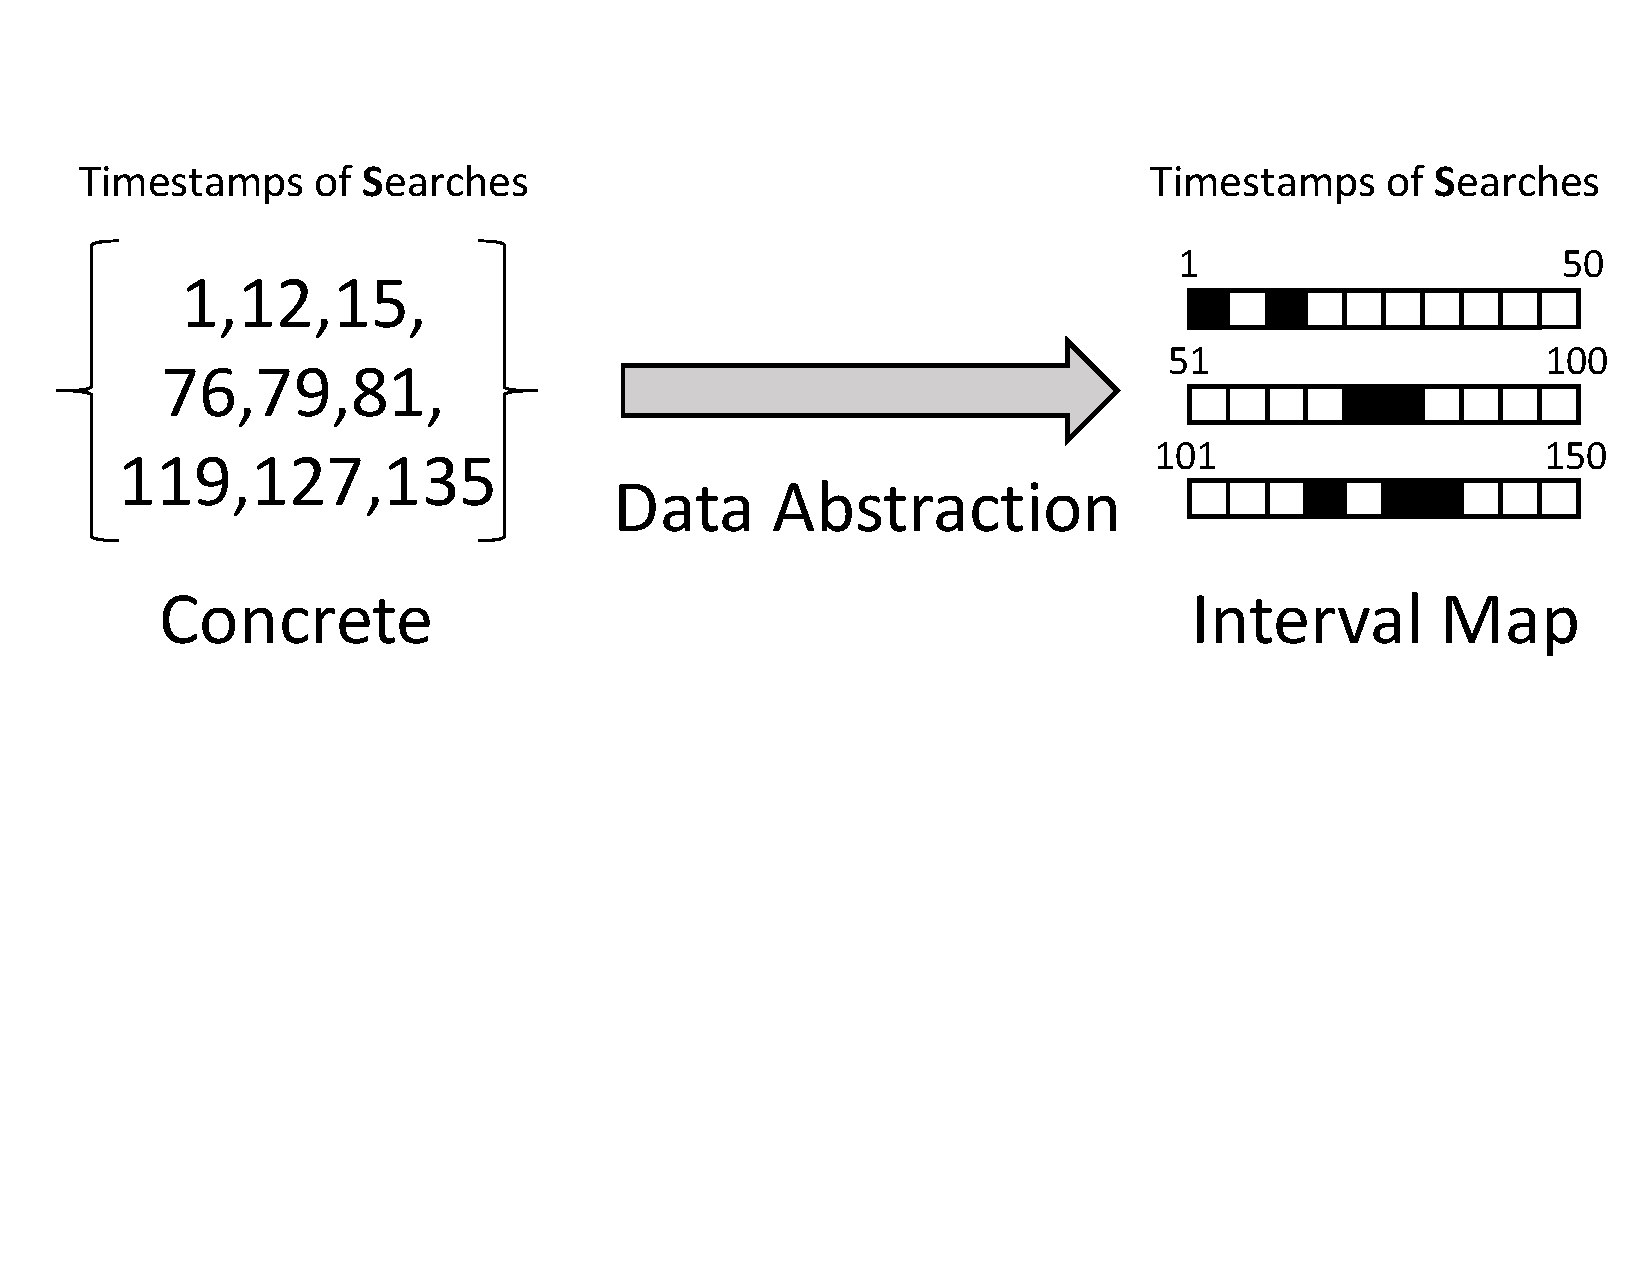
\includegraphics[clip, page=1,width=\columnwidth]{graphs/motivation.pdf}
    \vspace{-3.5cm}
    \caption{Intervals are a compact over-approximation of the timestamps of 
    searches.}
    \label{fig:dabstraction}
  \end{subfigure}
  %
  \begin{subfigure}{\columnwidth}
    \vspace{-0.5cm}
    \includegraphics[clip, page=2,width=\columnwidth]{graphs/motivation.pdf}
    \vspace{-2.5cm}
    \caption{SR*P will only match those users that search, possibly read
      some reviews, and finally, purchase a product.  Predicate abstraction
      exploits the selectivity of one predicate (most users do not purchase) to
      efficiently over-approximate users that match SR*P.}
    \label{fig:pabstraction}
  \end{subfigure}
  \caption{Examples illustrating the core intuitions underlying data and 
  predicate abstraction.}
\end{figure}
      
 
Our approach is inspired by the concept of abstract 
interpretation~\cite{Cousot:1977,Graf:1997}.  
In particular, the {\em abstract filter} constraints are the result of
relaxing/coarsening in a conservative manner of the precise constraints enforced
by the pattern regarding which events form successful matches.  This suggests
future work can leverage the technique of abstract interpretation to optimize
other user defined aggregates as well, (i.e.\ to derive abstract filters meant 
to remove from the input those tuples that are guaranteed not to contribute to 
an output of interest).

% abstract interpretation provides a template for how  this optimization can be 
%extended to other udf running in the reducer stages of a map-reduce pipeline 

%(Results)
As previously mentioned, constructing and applying the abstract filter incurs a
series of overheads, most notably it requires a second pass over the data.
Nonetheless, if the reduction in data is significant, these additional costs are
balanced out by the dramatic speedup in the sorting/shuffling/pattern matching
phases which results in an overall decrease in both processing costs and
latency.  Our experimental evaluation shows up to 3 orders of magnitude
reduction in shuffled data as well as 1.23x average speedup in total processing
time for 2 workloads: i) telemetry analysis over the events produced by an
event-reporting infrastructure, and ii) repository analysis over the dataset of
events published by GitHub.  The reduction in total processing time is
especially important in multi-tenant clusters where clients are billed based on
the amount of computational resources they consume.

The contributions of this paper are:
\begin{itemize}
	\item We show how a significant class of complex event patterns can be 
	translated to relational queries such that they can benefit from decades of 
	progress in relational optimizations.
	\item We introduce the technique of {\em abstract pattern matching} in 
	order to minimize the sorting/shuffling costs of large scale mining of 
	patterns within map-reduce frameworks.
	\item We design {\em data and predicate abstractions} that allow us to 
	trade the precision of our approach (but not its soundness) for lower 
	overheads.
	%\item We highlight how the concepts of symbolic execution and abstract 
	%interpretation can be used to design similar optimizations for other 
	%user-defined reduce operators.
	\item We prototype our solution and show on an industrial benchmark that 
	it delivers significant reductions in the amount of data sorted/shuffled as 
	well as processing times.  
\end{itemize}


The rest of the paper is organized as follows: 
we further illustrate our approach and detail its design in 
sections~\ref{sec:mot_example} and~\ref{sec:design},
the related work is discussed in section~\ref{sec:rel_work},  
the choices we made in implementing our solution are explored in 
section~\ref{sec:implementation}, followed by the presentation of the results 
of our experimental evaluation in section~\ref{sec:evaluation}. 
Finally, section~\ref{sec:conclusions} gives our concluding remarks and 
comments on future directions.   









\section{Motivating example}
\label{sec:mot_example}

Consider an analytics task that mines influential reviews
within the click-stream of an e-commerce website consisting of events of type
``Search''(S), ``Read review''(R) and ``Purchase''(P). 
The mining task is informally described in terms of the pattern
SR*P. In other words, we desire a user interation where the user
searched for an item, read a sequence of reviews, before deciding to
purchase. In particular, we want the user to perform no other actions
between the search and purchase actions. 


The mining task is described in terms of the pattern SR*P, with each event 
variable annotated by its own guard:
\begin{align*}
\text{{\bf S}} \in \Ev&: \facc{S}{name} = ``S"
\\
\text{{\bf R}} \in \Ev&: 
\facc{R}{name} = ``R"
\vee
(\facc{R}{name} \neq ``R") . 
(\facc{R}{user} \neq \facc{S}{user})
\\
\text{{\bf P}} \in \Ev&: (\facc{P}{name} = ``P") . 
(\facc{P}{user} = \facc{S}{user}) . 
(\facc{P}{t} < \facc{S}{t} + t_{out}),
\end{align*}
where we consider as input an $\Ev$(name, t, user) relation with fields for 
event name, event timestamp and associated user id, and we use $.$ as a 
shorthand for the conjunctive operator. 
The pattern is described in terms of both selection predicates (for identifying 
the name of the event to be matched), as well as join predicates that make sure 
that the matched events are correlated by the id of the user that performed 
them and that the ``Purchase'' event occurs within a timeout $t_{out}$ from the 
``Search'' event. 
\begin{comment}
In addition, figure~\ref{fig:srp_pattern} presents the symbolic automata 
representation of the pattern, i.e.\ the state machine where each transition 
has an associated event variable and a corresponding guard.
\end{comment}

The typical execution plan of this task on a map-reduce framework is to first
group all events by user id, then sort them on time and finally run a pattern
matching engine to detect the desired sequence of events.
In this work we propose to greatly expand the array of possible execution plans
by taking advantage of the fact that a large class of patterns can be
equivalently expressed as SQL queries.
By doing so then one can leverage decades of progress in query optimization to
come up with more efficient query plans than the one outlined above.
For instance, we can express our example pattern as a SQL query as follows:
{\small
	\begin{verbatim}
	SELECT S.*, P.*
	FROM Ev S, Ev P
	WHERE S.time < P.time
	AND S.name == "S"   
	AND P.name == "P" AND P.time < S.time + t_out
	AND P.user == S.user
	AND NOT EXISTS ( 
	    SELECT * FROM Ev NR
	    WHERE NR.name != "R"
	    AND S.time < NR.time AND NR.time < P.time
	    AND NR.user == S.user ); 
	\end{verbatim}
}

The first part of the query enforces the fact that a successful match consists
of an event S followed within a timeout $t_{out}$ by an event P from the same 
user,
while the second part captures the fact that only R events are allowed to take
place in between these two events.
The final result of the query is a set of tuples, one per successful match,
consisting of the initial and final event in the match.

% Since the number of purchase events P are likely to be much lower than the 
%search
% or read review events, performing a broadcast join wrt.\ to the P events might
% prove to be the optimum execution plan for this pattern. One of the key 
%insights
% of this paper is that representing a pattern as a SQL query provides 
%significant
% query optimization opportunities.

% The class of patterns that we can currently translate into SQL are those whose
% automata have only cycles of constant length, ie. every repetition
% within a particular cycle should consist of the same number of events. 
% Note this class includes the overwhelming majority of patterns discussed
% in the literature of complex event processing systems as well as encountered
% within an industrial benchmark.

% While we acknowledge that for patterns with many transitions, whose
% corresponding queries involve many joins, the optimizer might find optimal the
% standard query plan based on the pattern matching engine,
% we argue that even in such cases one can still leverage the derived query to
% minimize the number of events that get grouped by and sorted before being fed 
%to
% the pattern matching engine.
% Ideally, only the events that will end up as part of a successful match should
% undergo this process.
In the following we discuss our approach for performing this pre-processing step
in a time and space efficient manner.  

We start by defining for each event variable $X$ of the pattern 
{\em symbolic sets} $\syms{X}$, which collect the values of $X$'s fields that 
are joined by the query, based on the input events matching its selection 
predicates (for transition R, we get two such symbolic sets $\syms{R}$ and 
$\syms{\oR},$ as its guard has two disjoint selection predicates.). 
\begin{align*}
\syms{S} 
&\coloneq 
\{ \tuple{\facc{S}{t}, \facc{S}{user}} \mid 
S \in \Ev: \facc{S}{name} = \text{``S''}
\}
\\
\syms{R} 
&\coloneq 
\{ \tuple{\facc{R}{t}} \mid 
R \in \Ev: \facc{R}{name} = \text{``R''}
\}
\\
\syms{\oR} 
&\coloneq 
\{ \tuple{\facc{NR}{t}, \facc{NR}{user}} \mid 
NR \in \Ev: \facc{NR}{name} \neq \text{``R''}
\}
\\
\syms{P} 
&\coloneq 
\{ \tuple{\facc{P}{t}, \facc{P}{user}} \mid 
P \in \Ev: \facc{P}{name} = \text{``P''}
\}
\end{align*}


We introduce a slicing operator that simplifies our
notation. Given a set $S$ of tuples $\tuple{s_1,s_2,\ldots,s_n}$ and
unary predicates $\phi_1, \phi_2, \ldots, \phi_n$, we define the
slicing operator:
$$\slice{S}{\phi_1, \phi_2, \ldots, \phi_n} =
\{\tuple{s_1,s_2,\ldots,s_n} \mid \bigwedge_{i=1}^{n}\phi_i(s_i)\}
$$ 
We will also represent $u_=(t)$ for the unary predicate that determines if
$t$ is equal to $u$, and $(l,u)_\in(t)$ for the unary predicate that
determines if $t$ is in the (open) time interval $(l,u)$.

Next, we re-write the query, first using comprehension syntax, 
and then using the slicing operator:
\begin{align*}
&
Q \coloneq 
\{ \tuple{\symv{s}, \symv{p}} \mid 
\symv{s} \in \syms{S},
\symv{p} \in \syms{P}: 
\\ 
&
\qqquad\quad\;\;
\facc{\symv{p}}{t} \in
(\facc{\symv{s}}{t} : \facc{\symv{s}}{t} + t_{out})\ .\ 
(\facc{\symv{p}}{user} = \facc{\symv{s}}{user})\ .\ 
\\
&\qqquad\quad\;\;
\neg
(\exists
\symv{nr} \in \syms{\oR} : 
\facc{\symv{nr}}{t} \in (\facc{\symv{s}}{t} : \facc{\symv{p}}{t})\ .\ 
(\facc{\symv{nr}}{user} = \facc{\symv{s}}{user})
)
\ \}
\\
&
\;\;\; \coloneq 
\{ \tuple{\symv{s}, \symv{p}} \mid 
\symv{s} \in \syms{S},
\symv{p} \in 
\slice{\syms{P}}
{(\facc{\symv{s}}{t}\,:\,\facc{\symv{s}}{t} + t_{out})_\in,
	\facc{\symv{s}}{user}_=}
: 
\\ 
&\qqquad\quad\;\;
\slice{\syms{\oR}}
{(\facc{\symv{s}}{t}\,:\,\facc{\symv{p}}{t})_\in,\; \facc{\symv{s}}{user}_=} 
= \emptyset  
\ \}
\end{align*}
\begin{comment}
where 
$\slice{\syms{P}}
{(\facc{\symv{s}}{t}\,:\,\facc{\symv{s}}{t} + t_{out}),
	\facc{\symv{s}}{user}}
$
denotes the slicing of $\syms{P}$ defined as:
\begin{align*}
\{ \symv{p} \mid 
\symv{p} \in \syms{P} : 
\facc{\symv{p}}{t} \in (\facc{\symv{s}}{t} : \facc{\symv{s}}{t} + t_{out})\ .\ 
(\facc{\symv{p}}{user} = \facc{\symv{s}}{user})
\},
\end{align*}
and similarly for
$\slice{\syms{\oR}}
{(\facc{\symv{s}}{t}\,:\,\facc{\symv{p}}{t}),\; \facc{\symv{s}}{user}}$,
with the latter allowing us to express the \texttt{NOT EXISTS} sub-clause as an 
emptiness test.
\end{comment}

\begin{comment}
\begin{align*}
\{ \symv{r} \mid 
\symv{r} \in \syms{\oR} : 
\facc{\symv{r}}{t} \in (\facc{\symv{s}}{t} : \facc{\symv{p}}{t})\ .\ 
(\facc{\symv{r}}{user} = \facc{\symv{s}}{user})
\},
\end{align*}



\begin{figure}[t]
\centering
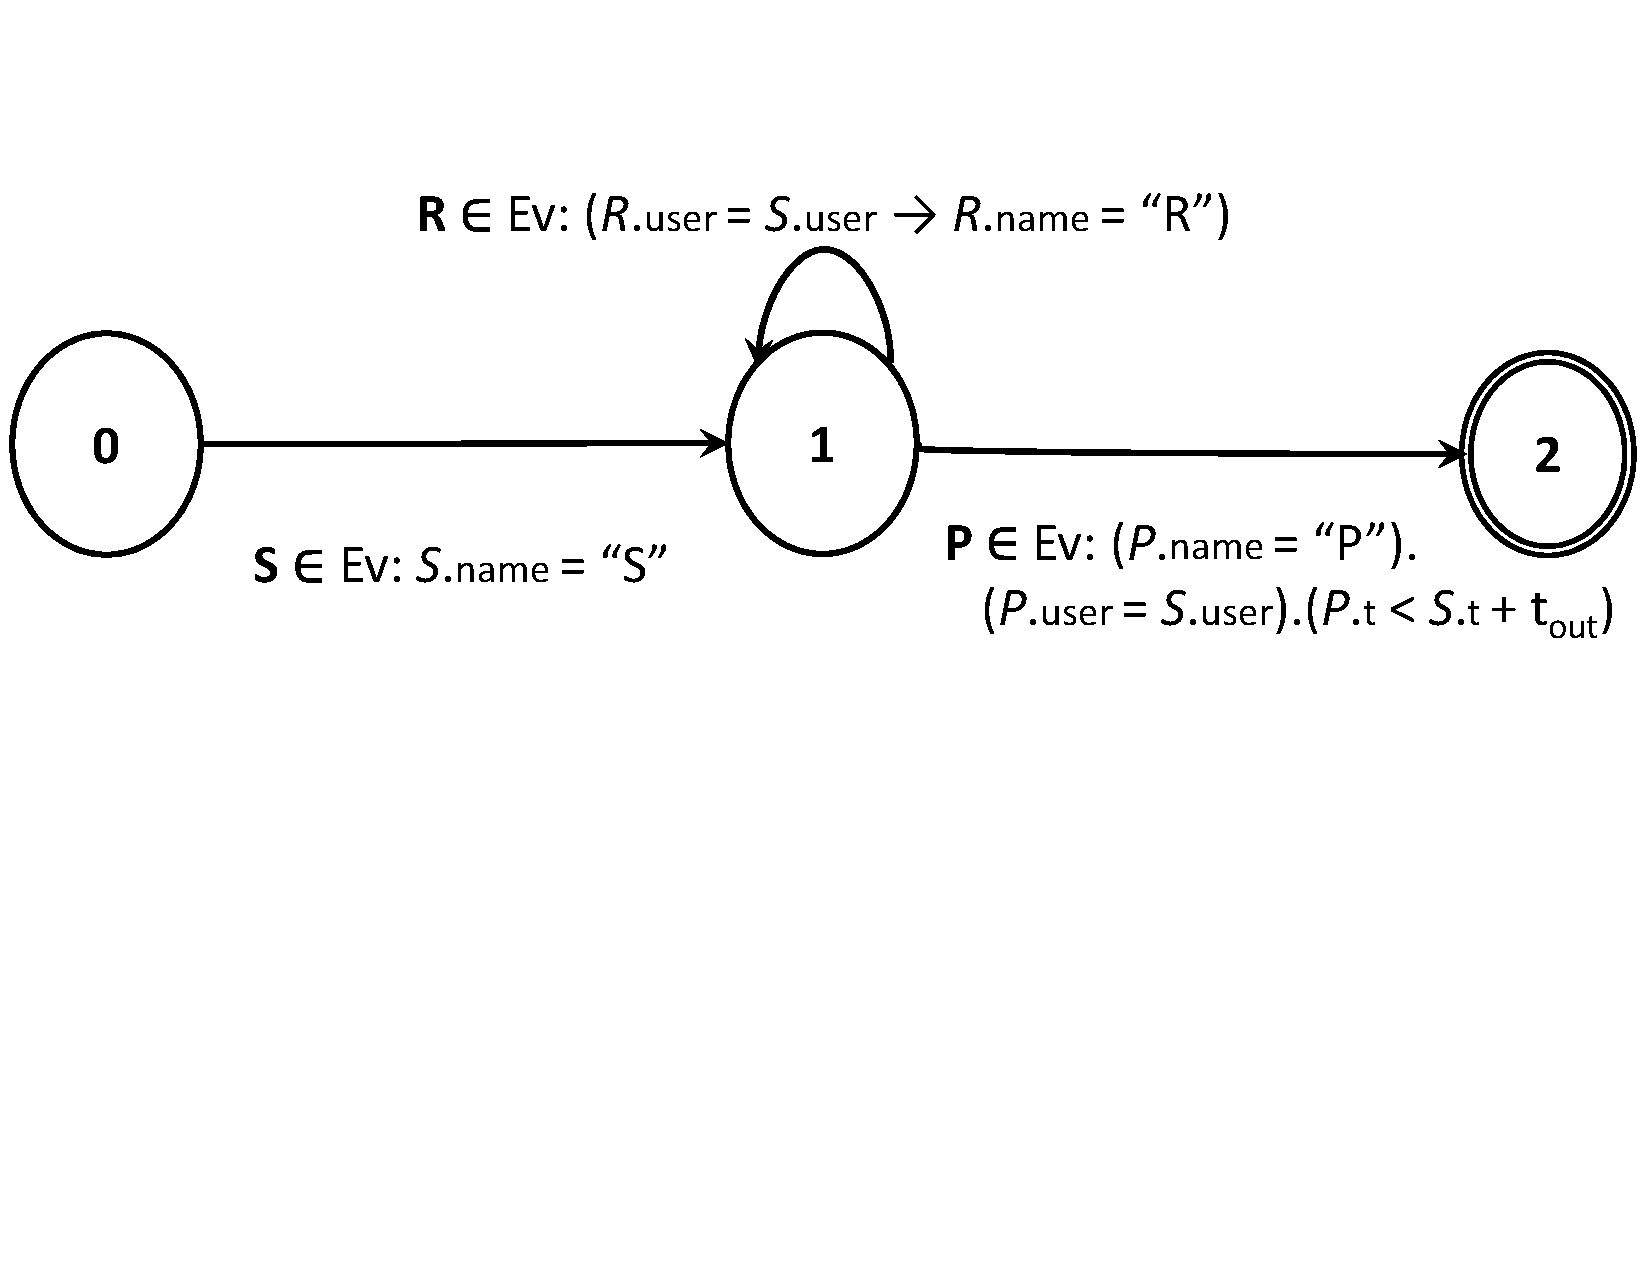
\includegraphics[clip, trim=0cm 10cm 0cm 3cm,width=\columnwidth]
{graphs/example_sm2.pdf}
\caption{Symbolic automata for the SR*P pattern.}
\label{fig:srp_pattern}
\end{figure}

\end{comment}

Each symbolic set, in concert with the slice operator let us remove events from
the input that are guaranteed not to participate in a successful match.
% and as such minimize the number of events being sorted and considered by the 
% pattern matcher, 
For this example pattern we get the following filters:
\begin{align*}
\precs{S}(\symv{s}) 
&\equiv  
\exists \symv{p} \in 
\slice{\syms{P}}
{(\facc{\symv{s}}{t}\,:\,\facc{\symv{s}}{t} + t_{out})_\in,
	\facc{\symv{s}}{user}_=} :\ 
\\
&\qquad\quad
\slice{\syms{\oR}}
{(\facc{\symv{s}}{t}\,:\,\facc{\symv{p}}{t})_\in,\; \facc{\symv{s}}{user}_=}
= \emptyset 
\\
\precs{R}(\symv{r}) 
&\equiv
\slice{Q}
{(-\infty\,:\,\facc{\symv{r}}{t})_\in,
	\texttt{true}, 
	(\facc{\symv{r}}{t}\,:\,\infty)_\in,
	\texttt{true}}
\neq \emptyset 
\\
%%%%%%%%%%%%%%%%%%%%%%%%%%%%%%%%%%%%%%%%%%%%%%
&\equiv
\exists \symv{s} \in 
\slice{\syms{S}}{(-\infty\,:\,\facc{\symv{r}}{t})_\in, \texttt{true}},
\\
&\quad
\exists \symv{p} \in 
\slice{\syms{P}}
{(\max(\facc{\symv{s}}{t},\facc{\symv{r}}{t})\,:\,\facc{\symv{s}}{t} + 
t_{out})_\in,
	\facc{\symv{s}}{user}_=}
: 
\\ 
&\qquad\quad
\slice{\syms{\oR}}
{(\facc{\symv{s}}{t}\,:\,\facc{\symv{p}}{t})_\in,\; \facc{\symv{s}}{user}_=} 
= \emptyset  
%%%%%%%%%%%%%%%%%%%%%%%%%%%%%%%%%%%%%%%%%%%%
\\
\precs{\oR}(\symv{nr}) 
&\equiv
\slice{Q}
{(-\infty\,:\,\facc{\symv{nr}}{t})_\in, 
	\facc{\symv{nr}}{user}_{\neq}, 
	(\facc{\symv{nr}}{t}\,:\,\infty)_\in, 
	\texttt{true}} 
\neq \emptyset 
\\
%%%%%%%%%%%%%%%%%%%%%%%%%%%%%%%%%%%%%%%%%%%%%%
&\equiv
\exists \symv{s} \in 
\slice{\syms{S}}{(-\infty\,:\,\facc{\symv{nr}}{t})_\in, 
\facc{\symv{nr}}{user}_\neq},
\\
&\quad
\exists \symv{p} \in 
\slice{\syms{P}}
{(\max(\facc{\symv{s}}{t},\facc{\symv{nr}}{t})\,:\,\facc{\symv{s}}{t} + 
t_{out})_\in,
	\facc{\symv{s}}{user}_=}
: 
\\ 
&\qquad\quad
\slice{\syms{\oR}}
{(\facc{\symv{s}}{t}\,:\,\facc{\symv{p}}{t})_\in,\; \facc{\symv{s}}{user}_=} 
= \emptyset  
%%%%%%%%%%%%%%%%%%%%%%%%%%%%%%%%%%%%%%%%%%%%
\\
\precs{P}(\symv{p}) 
&\equiv  
\exists \symv{s} \in 
\slice{\syms{S}}
{(\facc{\symv{p}}{t} - t_{out}\,:\,\facc{\symv{p}}{t})_\in,  
	\facc{\symv{p}}{user}_=} :\
\\
&\qquad\quad
\slice{\syms{\oR}}
{(\facc{\symv{s}}{t}\,:\,\facc{\symv{p}}{t})_\in,\; \facc{\symv{p}}{user}_=}
= \emptyset,
\end{align*}
which when applied to their corresponding symbolic set will retain only those 
events that contribute to the output of $Q$.
We detail the procedure for generating these precise filters from the 
relational query expressing the pattern in 
section~\ref{sec:prec_filter_generation}. 

Because evaluating these filters would in many cases be as expensive as 
computing
the complete result $Q$, we use them only as a starting point for deriving a set
of {\em abstract filters}, as a ``relaxed'' version of these
{\em precise filters}, but that can be applied with low processing and 
communication costs.
We do so by employing a series of {\em data and predicate abstractions} 
that generate conservative versions of the original filters.

\newcommand{\NotExistsP}{\ident{NotExistsP}}
\newcommand{\PrecedesP}{\precs{S}}
\newcommand{\PrecedesPP}{\omega_S}
\newcommand{\PrecedesPPP}{\psi_S}
\newcommand{\PrecedesPPPP}{\upsilon_S}


\newcommand{\interval}[1]{\lfloor #1 \rceil}
\newcommand{\uinterval}[1]{\lceil #1 \rfloor}
\newcommand{\hashid}[1]{\# #1}

 We showcase our techniques on the filter corresponding to the S event 
variable,
 which highlights the fact that the Search events in the output are 
those  
 that have only Read-review events by that same user between themselves and the 
 next Purchase 
 event occurring within a $t_{out}$ window of time.

\begin{comment}
we first complement in order to obtain the set of "Search" events that we 
want discarded.
\begin{align*}
\PrecedesP(\symv{s}) 
&\equiv  
\forall \tuple{\facc{\symv{p}}{t}, \_} \in 
\slice{\syms{P}}
{(\facc{\symv{s}}{t}\,:\,\facc{\symv{s}}{t} + t_{out}),
\facc{\symv{s}}{user}} :\ 
\\
&\qquad
\slice{\syms{\oR}}
{(\facc{\symv{s}}{t}\,:\,\facc{\symv{p}}{t}),\; \facc{\symv{s}}{user}}
\neq \emptyset 
\end{align*}
\end{comment}

%User's that search for a product must (i) optionally read a review and
%ultimately, (ii) purchase a product \emph{within} a window of $t_{out}$
%time. 

\emph{Data abstraction} provides time and space efficient
representations for symbolic sets $\syms{S}$ and $\syms{\oR}$.  
For example, one could
abstract over time and coarsen timestamps $t$ into time intervals
$\interval{t}$.  Then, the time dimension of sets $\syms{S}$, $\syms{\oR}$ could
be efficiently encoded and queried as interval maps (i.e., bit vectors where
each bit corresponds to a time interval and a set bit would denote the fact that
an event has occurred within the corresponding interval).  Using this
abstraction the filter becomes:
\begin{align*}
\PrecedesP^{\interval{t}}(\symv{s}) 
&\equiv  
\exists \symv{p} \in 
\slice{\syms{P}}
{\interval{\facc{\symv{s}}{t}\,:\,\facc{\symv{s}}{t} + t_{out}},
	\facc{\symv{s}}{user}} :\ 
\\
&\qquad\quad
\slice{\syms{\oR}}
{\uinterval{\facc{\symv{s}}{t}\,:\,\facc{\symv{p}}{t}},\; 
	\facc{\symv{s}}{user}}
= \emptyset 
\end{align*}
where in order to maintain conservativeness (i.e.,
$\PrecedesP \rightarrow \PrecedesP^{\interval{t}} $) we must over-approximate
the $\facc{\symv{s}}{t}:\facc{\symv{s}}{t} + t_{out}$ range but
under-approximate the $\facc{\symv{s}}{t}:\facc{\symv{p}}{t}$ interval.  Thus,
in order to be sound (and, depending on the filter) data abstractions may
provide both over- and under- approximations of the original sets.


There are many different ways to approach data abstraction.  For example, 
hashing
is one approach to abstract over sets.  If we use a compact representation of
sets $\syms{S}$, $\syms{\oR}$ that stores time information only per user hash
bucket as opposed to individual user ids, then the resulting abstract filter:
\begin{align*}
&
\PrecedesP^{\hashid{user}}(\symv{s}) \equiv 
\exists \symv{p} \in 
\slice{\syms{P}}
{(\facc{\symv{s}}{t}\,:\,\facc{\symv{s}}{t} + t_{out}),
	\hashid{\facc{\symv{s}}{user}}} :\ 
\\
&\qqquad\qquad\quad\;\,
\slice{\syms{\oR}}
{(\facc{\symv{s}}{t}\,:\,\facc{\symv{p}}{t}),\; 
	\hashid{\facc{\symv{s}}{user}}}
= \emptyset 
\end{align*}
does not satisfy our safety requirement 
(i.e.\ $\PrecedesP \nrightarrow \PrecedesP^{\hashid{user}}$).
This happens because hashing can only provide over approximations of sets while,
in order to ensure conservativeness, the abstractions used for this filter need
to provide both over and under approximations.
While there are several ways to address this issue (for an alternative solution 
see section~\ref{sec:data_abstraction}), 
in the following we show how {\em predicate abstraction} can alleviate the 
problem.


Predicate abstraction encompasses a set of re-writings 
that relaxes the filter by discarding those constraints that cannot be safely
or efficiently abstracted over.
For instance, our filter could be weakened into:
\begin{align*}
&
\PrecedesPPP(\symv{s}) \equiv 
\slice{\syms{P}}
{(\facc{\symv{s}}{t}\,:\,\facc{\symv{s}}{t} + t_{out}),\; 
	\facc{\symv{s}}{user}}
\neq \emptyset,
\end{align*} 
which eliminates only those search events that are not followed by a purchase
event within $t_{out}$, and was obtained from the base case of
the existential quantifier in $\PrecedesP$.
Since this version only requires over-approximation, one can safely use hashing
to abstract over the user id dimension of $\syms{P}$, i.e.\ 
$\PrecedesPPP \rightarrow \PrecedesPPP^{\hashid{user}}$, where
\begin{align*}
&
\PrecedesPPP^{\hashid{user}}(\symv{s}) \equiv 
\slice{\syms{P}}
{(\facc{\symv{s}}{t}\,:\,\facc{\symv{s}}{t} + t_{out}),\; 
	\hashid{\facc{\symv{s}}{user}}}
\neq \emptyset .
\end{align*}

Moreover, predicate abstraction also reveals the well known Bloom
join algorithm as an instance of our approach, wrt.\ the join
predicate $\facc{P}{user} = \facc{S}{user}$ from the original query. 
This becomes apparent if we ignore time in the filter above:
\begin{align*}
&
\PrecedesPPP^{\hashid{user}}(\symv{s}) \equiv 
\slice{\syms{P}}{*, \hashid{\facc{\symv{s}}{user}}}
\neq \emptyset,
\end{align*}
and we use a Bloom filter to implement 
$\slice{\syms{P}}{*, \hashid{\facc{\symv{s}}{user}}}$.
More importantly, it highlights the fact that one can use data and predicate 
abstraction to explore the entire spectrum of abstract filters, and make the 
choice between precision vs overheads on a case by case basis.
We discuss additional scenarios where predicate abstraction proves
beneficial in section~\ref{sec:pred_abstraction}.




\begin{comment}
\\
&
\NotExistsP(t_S, user_S) \coloneq 
E_P(t_S..t_S+t_{out}, user_S) = \emptyset

These filters are designed to be applied independently over the input without
the need to perform any joins, group by's or order by's.
More importantly, in a map-reduce framework they can be performed with minimal
communication overhead.


- interval map may use different granularities in different regions of the
timeline, i.e. finer granularity in regions with higher probability of events
\end{comment}





































\section{Related Work}

(*) Pattern matching over out-of-order event series.

(*) Distributed pattern matching

(*) Stream processing engines optimizations

(*) Pattern matching algorithms optimizations
\section{Design}

We consider patterns specified as a symbolic finite automata where each
transition has a guard (propositional formula) whose predicates test the
currently considered event against constants as well as events matched by
preceding transitions.
   
Pattern matching algorithms require data sorted on time.
In a map-reduce framework this makes the reducer the main bottleneck of the
analysis, both at the network level (large amounts of shuffled data) and at
the processing level (in case of data-skew).



We propose to significantly reduce the amount of data fed into the pattern
matcher (reducer) by dropping in a map phase all the events that cannot take
part in a successful match.

To do so we design a set of filters that while conservative, closely match the
semantics of the patterns analyzed.
We propose three levels of abstraction.
The first enforces the join constraints between different transitions as
expressed by join predicates within the transition guards.
The second one further imposes time windowing constraints (all events of a
successful match must occur within a timeout of the first event in the match).
Finally the last one enforces ordering constraints between {\em consecutive}
transitions of the pattern.

In our approach we leverage the fact that a large class of symbolic finite
automata fit within the fragment of star-free languages which
have a corresponding FOL formula (possibly with counting quantifiers).
Whenever that is not the case we can narrow the scope of our filters to the
sections of the pattern that do.
 
We relax these FOL formulas to produce precise filters, one per transition, 
that can be evaluated independently on each mapper.
Finally we further coarsen these filters to a set of relaxed filters
that can be collected and tested in a time and space efficient manner (eg. bloom
filters, time-interval maps).

We explore the trade-offs involved in the overheads incurred in building the
filters and their accuracy. 








\section{Implementation}
\label{sec:implementation}

\begin{figure}[tp]
\centering
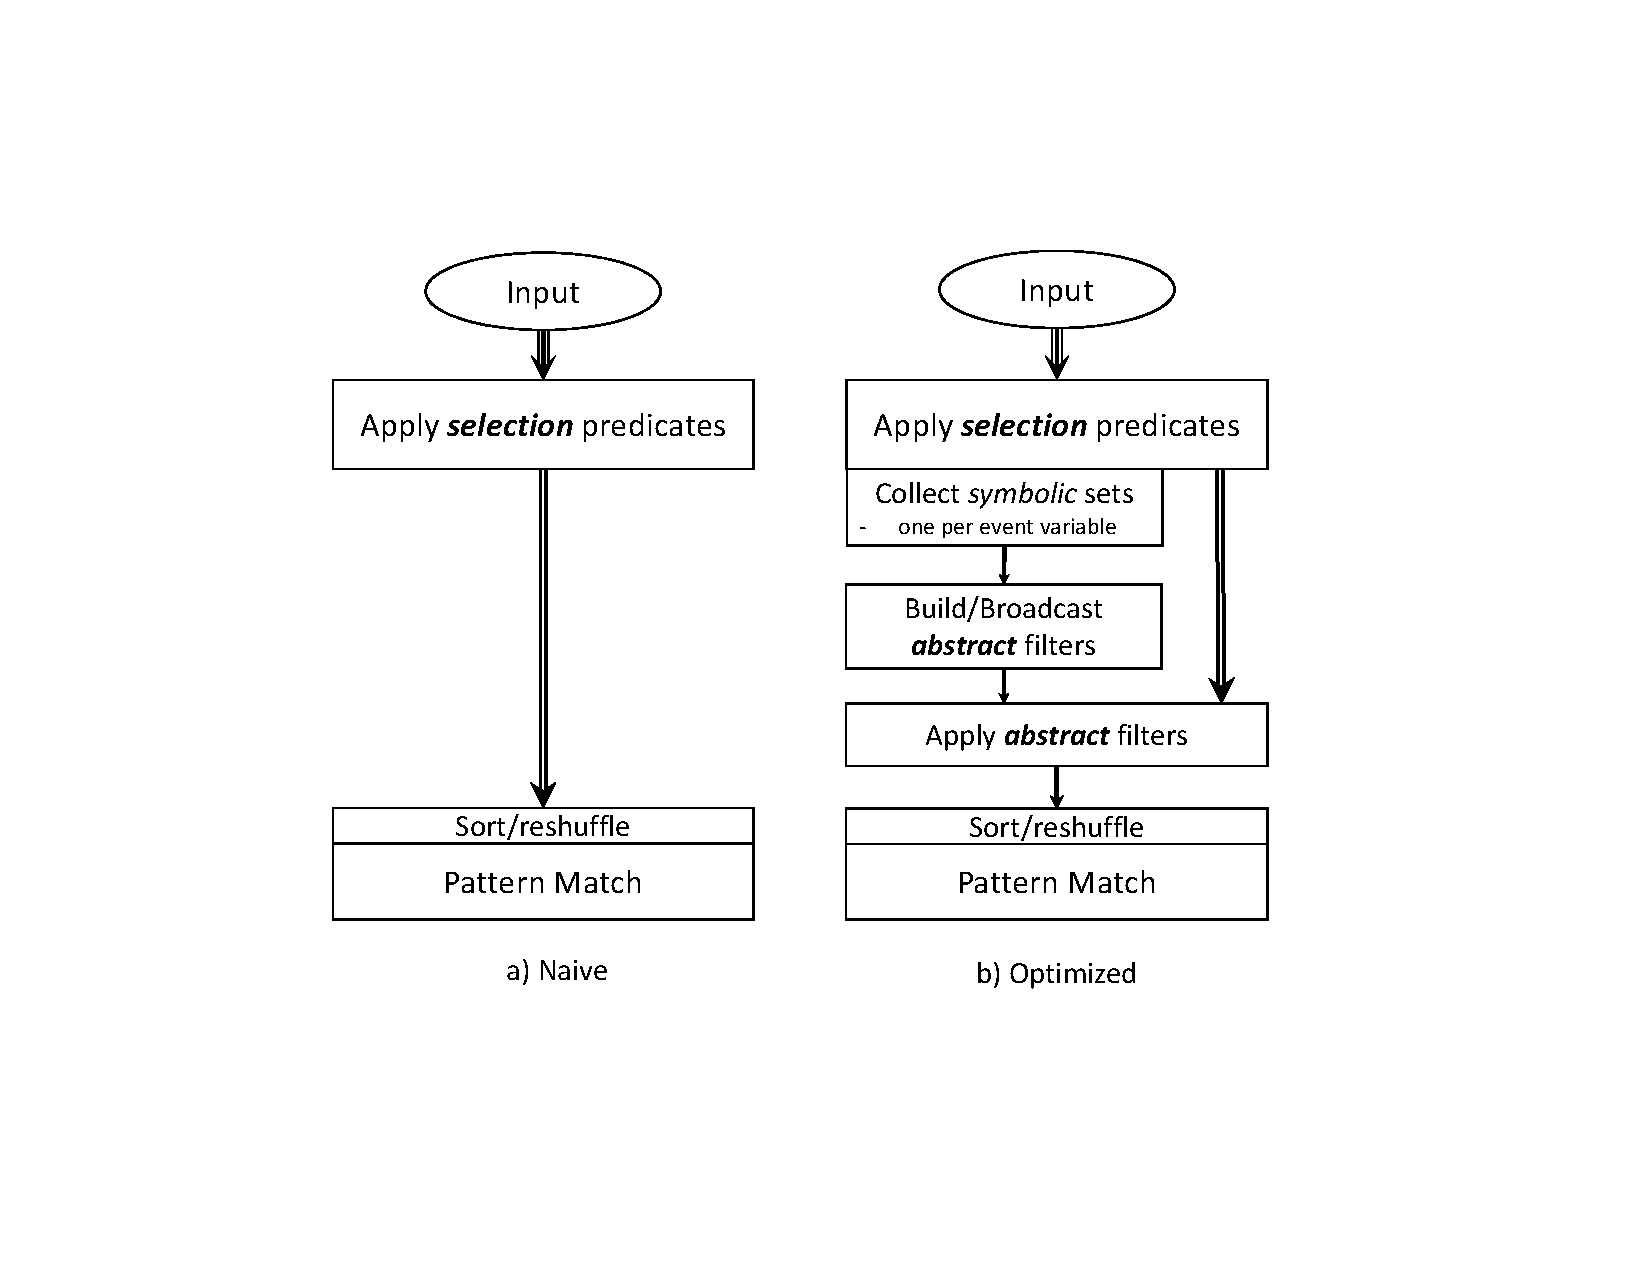
\includegraphics[clip, trim=5.6cm 4.5cm 6.3cm 4.2cm, 
width=0.45\textwidth]{graphs/query_plan.pdf}
\caption{Naive (a) and optimized (b) execution plans for performing pattern 
matching on a map-reduce platform.}
\label{fig:query_plan}
\end{figure}


In the following we detail how we implemented our solution for speeding up 
large scale event series pattern matching on top of the 
Cosmos/Scope~\cite{Chaiken:2008} map-reduce framework.
We recall that the standard way of performing event-series pattern matching in 
such frameworks is to first remove all the events that do not match any of the 
selection predicates specified by the pattern, and then to sort on 
time/reshuffle the remaining events and finally process them using a pattern 
matching engine (see figure~\ref{fig:query_plan}a).

Our solution significantly extends the amount of data that gets filtered out 
during the preprocessing stage by constructing {\em abstract} filters which 
also enforce the join predicates occurring in a pattern (as opposed to just the 
selection predicates).
To do so, we first collect in a parallel fashion a symbolic/abstract (event) 
set for each event variable of the pattern, then we union these sets across all 
partitions of the input and we use them to build the abstract filters by 
enforcing the join predicates between event variables. 
We then broadcast the abstract filters back to the preprocessing nodes and have 
them apply the abstract filters over the output of the initial 
selection-predicate based filter. 
Finally, the remaining events are sorted/reshuffled, just like in the standard 
approach and processed by the pattern matching engine. The entire execution 
plan is outlined in figure~\ref{fig:query_plan}b.


In implementing the execution plan in figure~\ref{fig:query_plan}b,
we make use as much as possible of the relational constructs and annotations 
provided by the Scope query language in order to maximize the potential for 
optimizations at the level of the entire data processing pipeline (for eg. we 
use native Scope to extract the event fields used in constructing the symbolic 
sets as well as to apply the filters that we build).
For operating with the set abstractions themselves we use the rich 
extensibility features of Scope, all the while providing hints to its query 
optimizer.

Even though the {\em abstract} filters have the potential to dramatically 
reduce the amount of data that gets sorted\allowbreak /\allowbreak 
reshuffled\allowbreak /\allowbreak pattern matched, 
constructing them introduces overheads both in terms of processing costs and 
latency.
In terms of processing costs we note that, while the construction of the 
symbolic sets can be done in the same pass as the selection-predicate based 
filtering, for applying the abstract filters we need a second pass over the 
data.
Nonetheless, since applying a filter is linear in the size of the input, this 
extra pass ends up being much cheaper than sorting on time the same input, and 
if the reduction ratio of the filter is considerable then applying it results 
in a net win. 
   
In terms of latency, our approach also introduces an extra reduction phase as 
required for aggregating the symbolic sets computed on each partition to a 
particular node where we can propagate the constraints specified by join 
predicates in order to obtain the abstract filters.
This is also followed by a broadcast phase that delivers the abstract filters 
back to the nodes processing the input stream.
In order to minimize the penalty in latency incurred by these two steps we 
limit the size of the abstract filters to the order of megabytes and we exploit 
the algebraic properties of the operators of the set abstractions that we use 
in order to optimize the aggregation (i.e.\ we make use of a {\em recursive} 
user defined aggregates).





  
  
  
  

\begin{figure*}[t!]
\begin{small}
\begin{center}
\setlength\tabcolsep{4pt}
  \begin{tabular}{l | c c c c c c c c c c c c c c c c c c}
    \hline
    Query & 
    A1 & A2 & A3 & A4 & A5 & A6 & A7 & A8 & A9 & A10 & A11 & A12 & A13 & A14 &
    A15 & G1 & G2 & G3 
    \\ \hline 
    No.\ of Transitions & 
    2 & 3 & 3 & 2 & 3 & 2 & 3 & 5 & 6 & 25 & 4 & 5 & 3 & 13 & 18 & 3 & 4 & 2 
    \\
    Has Union & 
     &  &  &  &  &  &  &  & $\checkmark$ & $\checkmark$ &  & $\checkmark$ &  &
     $\checkmark$ & $\checkmark$ & $\checkmark$ &  &
    \\
    Has Kleene Star & 
     &  &  &  &  &  &  &  & $\checkmark$ & 
     \begin{tabular}[c]{@{}c@{}}$\checkmark$\\(group)\end{tabular} &
     $\checkmark$ & $\checkmark$ & $\checkmark$ & $\checkmark$ & 
     \begin{tabular}[c]{@{}c@{}}$\checkmark$\\(group)\end{tabular} &  &
     $\checkmark$ &
    \\
    Has SecondaryKey & 
     & $\checkmark$ & $\checkmark$ & $\checkmark$ & $\checkmark$ &  &  & $\checkmark$ &
     $\checkmark$ & $\checkmark$ &  &  &  & $\checkmark$ &  &  &  & $\checkmark$
    \\
    Input Size(GB) & 
    216 & 321 & 477 & 264 & 1361 & 180 & 148 & 158 & 1167 & 587 & 234 & 1167 &
    286 & 366 & 141 & 593 & 593 & 85
    \\
    \hline
  \end{tabular}
\vspace{-10pt}
\end{center}
\end{small}
\caption{Workload characteristics}
\label{tab:workload}
\end{figure*}



\section{Evaluation}
\label{sec:evaluation}

We tested our approach on 2 workloads:
i) an internal Microsoft production system, consisting of 15 patterns (A1-15) matched over telemetry events
collected within a 2 hour interval, and 
ii) GitHub, performing repository analytics (patterns G1-3) over the GitHub
dataset consisting of events collected over a 5 years period.
All transitions in a pattern have a main key constraint, i.e.\ all events in a
match should belong to the same join condition for the Microsoft workload, or the same
repository for the GitHub patterns, and a time constraint, i.e.\ all events 
considered should occur within a timeout from the initial event in the match.
In addition, 9 patterns also have a secondary key constraint between some of
their transitions.
The characteristics of our workload are summarized in figure~\ref{tab:workload}.
The queries that we experiment with have up to 25 transitions and make use of
both {\em union} and {\em Kleene star}. 
In particular, queries A10 and A15 apply the Kleene star over a sub-pattern as
opposed to a single query variable.


We experimented on a virtual cluster consisting of 85 nodes as part of the 
Cosmos~\cite{Chaiken:2008} infrastructure.
We assess the benefits provided by our approach in terms of 
the ratio of input events vs selected events, 
the total execution time across the processing nodes of the cluster,
and the time it takes to complete the query (latency).
In measuring the data reduction provided by our abstract filters for a specific
query we use as baseline only the events from the input stream that satisfy the
selection predicates of some transition in the query. 
This way we can evaluate our approach in isolation from the standard technique
of pushing selection predicates into the scan operator of a query. 
The resulting amount of data to be processed by each query is detailed in
figure~\ref{tab:workload}.
Finally, we use query A5 to highlight the individual filtering potential
of different join predicates, as well as their sensitivity wrt.\ the amount of
state dedicated to their abstract representation.

Note that we also do not measure the cost to run the pattern matching engine and
so our overall system processing time and latency numbers are conservative
estimates of a production installation of our system.

\begin{figure}[t!]
\centering

\begin{subfigure}[t]{\columnwidth}
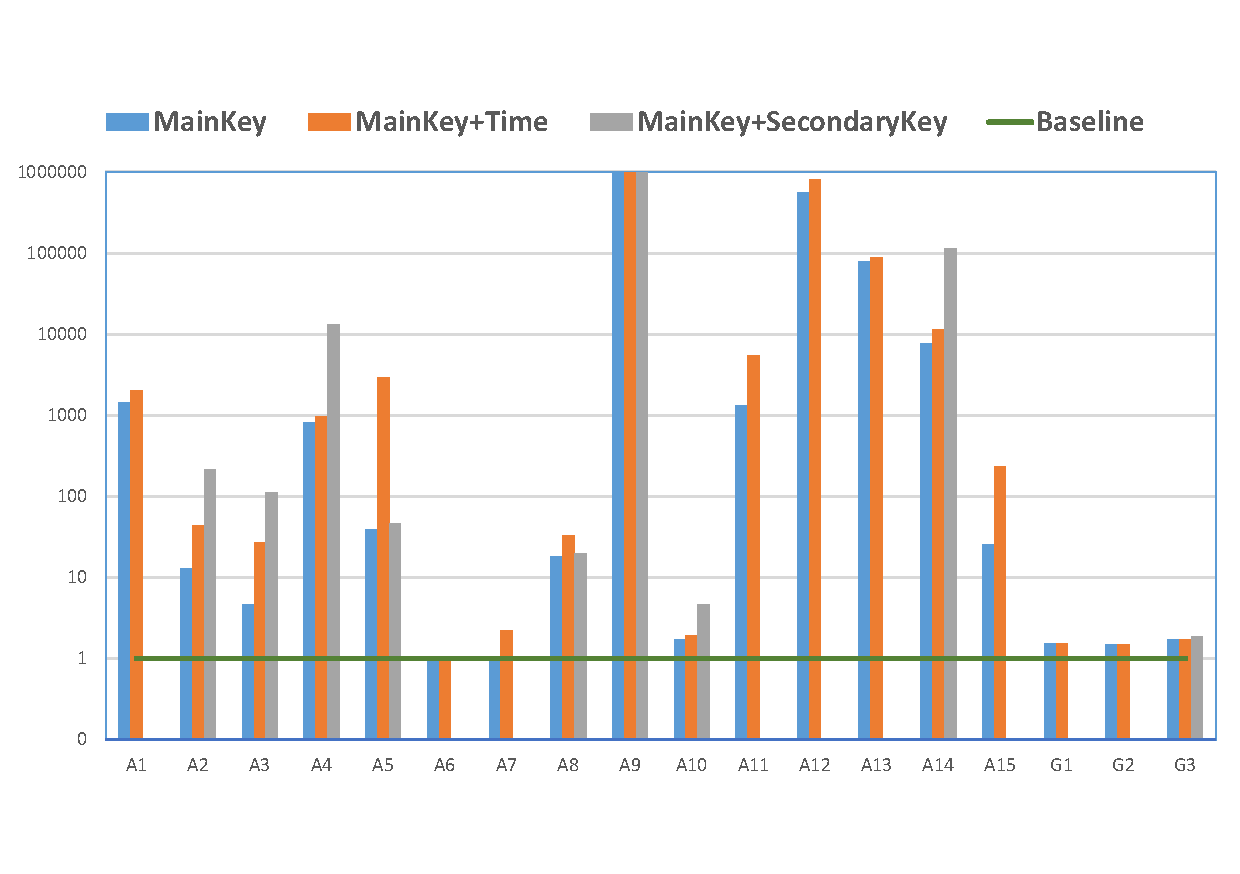
\includegraphics[clip, trim=0.3cm 1.6cm 0.4cm 1.6cm,
width=\columnwidth]{graphs_data_red.pdf}
\caption{Processed data reduction}
\label{fig:data_red}
\end{subfigure}
~
\begin{subfigure}{\columnwidth}
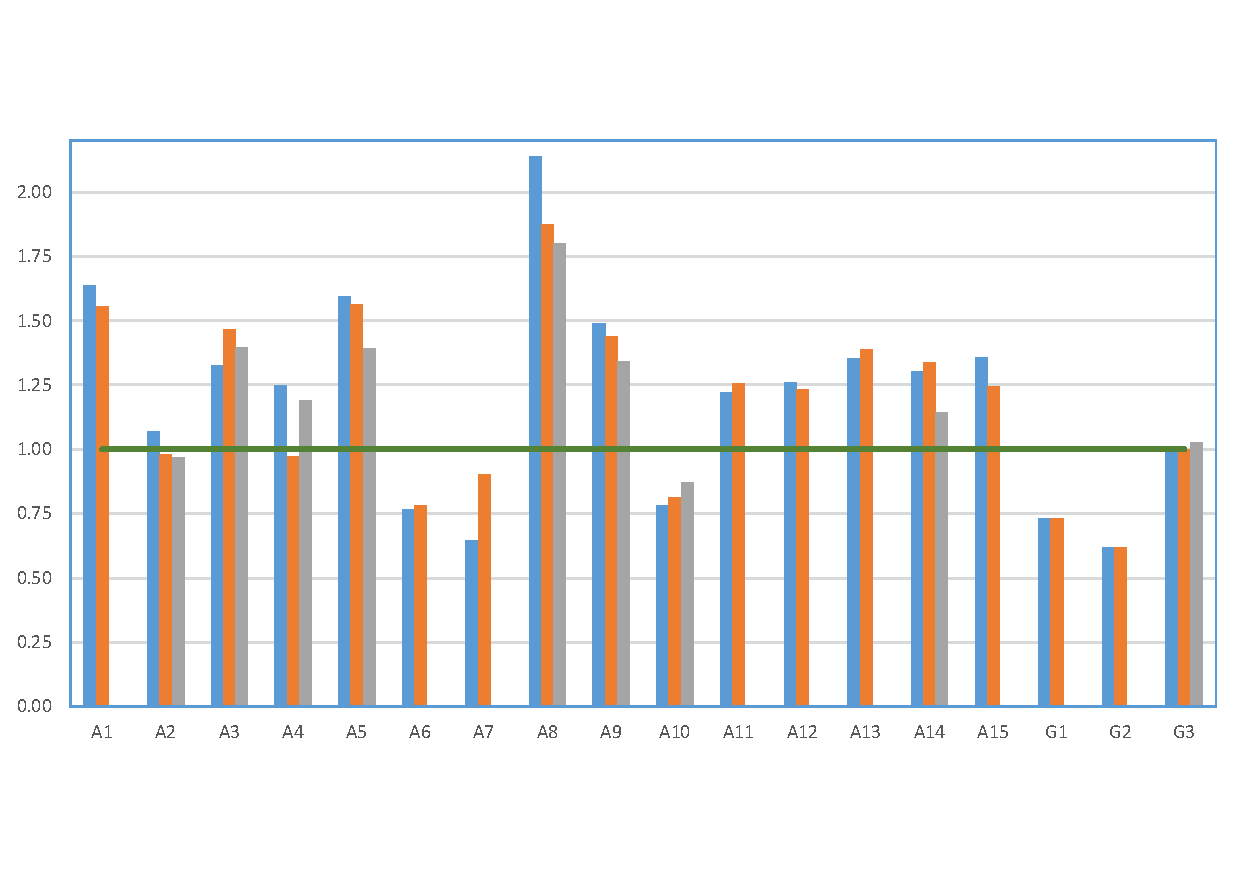
\includegraphics[clip, trim=0.3cm 2cm 0.4cm 1.8cm,
width=\columnwidth]{graphs_processing_red.pdf}
\caption{Processing time speedup}
\label{fig:processing_red}
\end{subfigure}
~
\begin{subfigure}{\columnwidth}
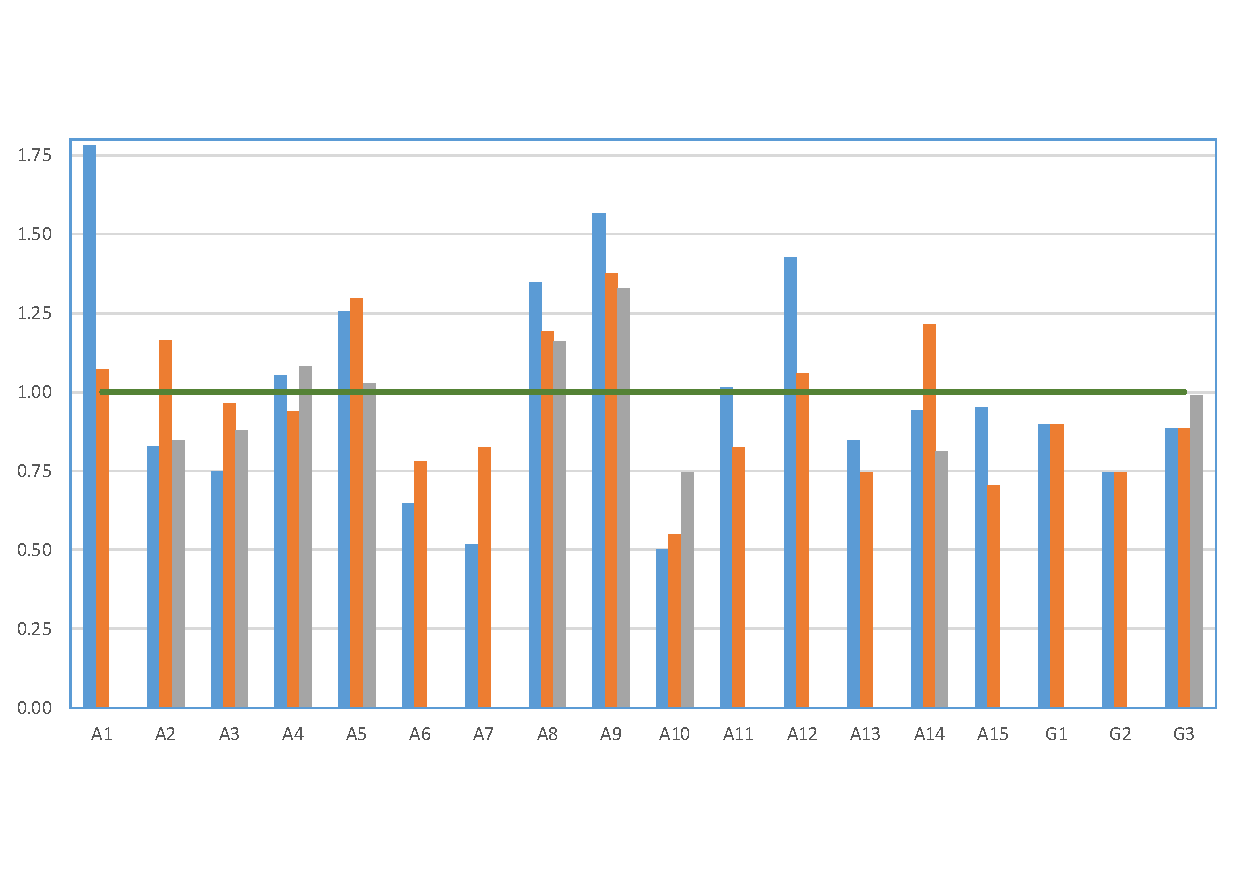
\includegraphics[clip, trim=0.3cm 2cm 0.4cm 1.8cm,
width=\columnwidth]{graphs_latency_red.pdf}
\caption{Latency speedup}
\label{fig:latency_red}
\end{subfigure}

\caption{Reduction ratios of processed data and processing speedups when using
abstract filters wrt.\ the corresponding baseline measures.}
\end{figure}


\subsection{Processed data reduction}

In order to establish the raw potential of our approach we look at the amount of
data that is discarded by the abstract filters that we build.
The baseline consists only of events whose type matches the event
type of a transition in the query.

Figure~\ref{fig:data_red} shows on a logarithmic scale the ratio between the
data processed by the baseline approach and the data processed by our solution
when considering different join predicates for building the abstract filters.
In particular, we look at three types of join predicates: those referencing
the main join key of the query (MainKey), those imposing constraints on the
timestamp of matching events (Time), and those referencing a secondary join key
(SecondaryKey).
We report the results provided by the MainKey filter as well as its combination
with the Time and SecondaryKey filter (for queries with joins on a secondary
key).
 
For 12 out of the 18 queries in our workload we obtain at least a 10x reduction
in the amount of data that has to be considered by the pattern matcher, with 3
of them ending up processing 5 orders of magnitude less data.
The other 6 queries exhibit modest or no data reduction. This is mainly due to
the precision lost by our abstract filters, as well as the fact that not all
join predicates from a query can be efficiently abstracted over. 

While incorporating extra join predicates in the abstract filters leads to
further savings, it is dependent on the query and the stream of events which
additional join predicate would provide the most benefits.
In our workload we observe that adding the Time filter for queries A5 and A8 
provides the biggest improvement while for queries A2-4, A10, A14 and G1 the
SecondaryKey filter is more advantageous. 
Due to this variability one has to decide on a query by query basis which join
predicates to use and how much state to allocate for them within the abstract
filter.
For our workload we assign to the MainKey, Time and SecondaryKey filters between
16KB and 4MB, 8B and 180B, and 2B and 8B, respectively.
This allocation has been chosen under the constraint of a total size for the
abstract filter in the order of megabytes and while considering the
particularities of queries, for example, we take into account the fact that a
query with a large timeout window would not benefit from a finegrained Time
filter.





\subsection{Abstract filter size vs reduction ratio}

We vary the size of the abstract filter that we build as well as its
configuration in order to asses the impact on the reduction ratio it provides.
In particular, we experimented for query A5 with filters of sizes between 1024
to 8192KB and with a granularity for the MainKey filter between 65K to 2M
distinct values. For each abstract filter size and MainKey granularity we devote
the rest of available space to either the Time or the SecondaryKey filter.
Since the filters we build are multiplicative in their composition, the
granularity afforded to the Time and SecondaryKey filters varies between 4 and
1024 distinct values depending on the granularity of the MainKey filter as well
as the total size of the abstract filter.
In addition we record for reference the reduction in data achieved just by the
MainKey filter for its different configurations.

From the results presented in figure~\ref{fig:tradeoff} we conclude that for
query A5, MainKey+Time is the most effective configuration as it provides the
most reduction in the number of input events irrespective of the other
parameters of the abstract filter. As expected, the bigger the size of the
abstract filter the larger is the reduction rate achieved.
We also note that the distribution of state amongst the components of the
abstract filter is also important, as refining the granularity of only one of
its components while keeping the total size of the filter fixed can experience a
sweetspot beyond which the reduction rate is negatively impacted.
This is reflected in our results for the MainKey+Time configuration where the
512K granularity setting for the MainKey component outperforms the 2M setting
across all filter sizes.
The drop in the reduction rate is a consequence of the fact that the MainKey
filter reaches a plateau, beyond which increasing its granularity no longer
increases the reduction rate, while decreasing the granularity of the Time
filter is bound to decrease its filtering power.

There is also a knock-on effect between the different components of the abstract
filter, as a poor choice for the granularity of one component can inhibit the
filtering potential of the other components as well.
For example, in query A5 a too small granularity for the MainKey filter (65K
setting in figure~\ref{fig:tradeoff}) results in poor performance for the
SecondaryKey component as well, as it cannot cope with the large number of
events and their associated secondary keys it needs to discriminate between.
Notably, the Time component is less susceptible to this issue. 






\begin{figure}[tp]
	\centering
	
	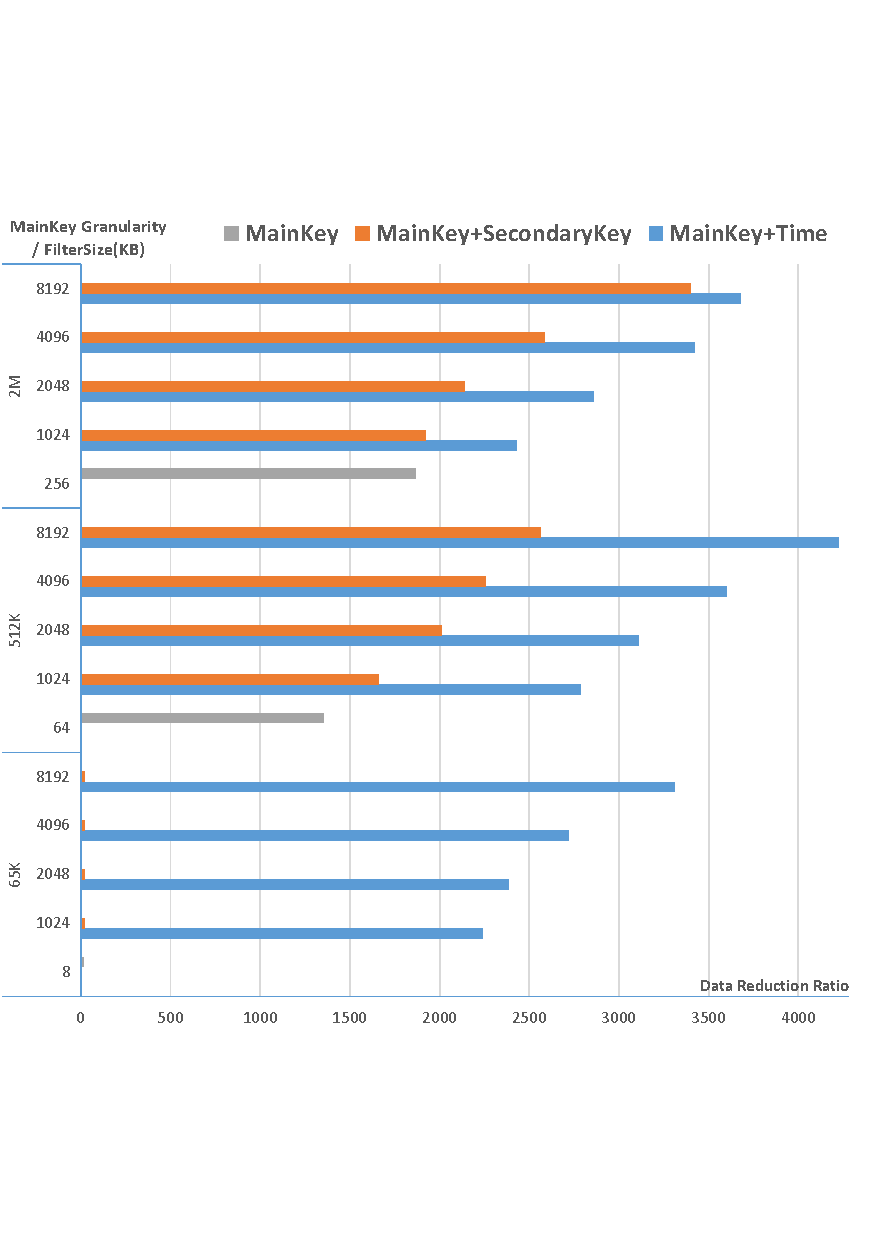
\includegraphics[clip, trim=0cm 3.5cm 0.3cm 3.7cm,
	width=\columnwidth]{graphs_A5_tradeoff.pdf}
	\caption{Tradeoff for query A5 between filter size (1024KB-8192KB) and data
		reduction for different filter configurations and with different 
		granularities
		for the MainKey filter (65K,512K,2M).}
	\label{fig:tradeoff}
\end{figure}

\subsection{Total processing time speedup}

In the following we look at the total processing cost across all nodes in the
cluster.
This is a particularly relevant metric for cluster setups that allow workload
consolidation or data centers that charge users based on total number of
``processing hours'' consumed.
Figure~\ref{fig:processing_red} shows speedups of 1.25x to 2.14x for 11 out of
the 18 queries, while 5 patterns experience slowdowns of at most 0.62x.
The slowdowns are a consequence of performing an additional pass over the input
in order to build the abstract filters, with little or no benefit in terms of
discarded events.

In order to highlight the tradeoffs of our approach we break down the {\em
baseline} execution of a query into the time it takes to 
i) read and sort the data, and 
ii) perform the reduction step.
On the other hand for our technique we look at the time it takes to 
i) read the data, 
ii) build the symbolic state associated with each transition,
iii) reduce the symbolic state associated to each transition down to an abstract
filter for the entire query and broadcast it back to every mapper,
iv) filter the input events based on the abstract filter, and
v) perform the reduction step over the remaining events. 
For both the baseline and our approach, the final reduction 
step just collects the events from the mappers, but does not perform the 
pattern matching.
We made this choice in order to asses our solution independent
from a particular implementation of the pattern matching operator
and to underscore the fact that any of the existing complex event processing 
systems could benefit from our approach.
Moreover, as the cost of pattern matching is typically proportional to the size 
of the input, taking it into consideration would more negatively impact the 
baseline approach than ours. 

By discarding some of the input events our solution cuts the cost
of the sorting and reduction phases when compared to the baseline approach,
while adding the overhead of building and applying the abstract filters.
When the number of events removed is significant this leads to an overall lower
processing time as can be seen in figure~\ref{fig:breakdown}.
Since every join predicate included in the abstract filter incurs additional
costs when building and applying the filter, to maximize performance one should
consider only the smallest/cheapest set of predicates able to filter the input
down to the order of gigabytes/tens of gigabytes.


In particular the additional reduction in data provided by the
Time filter for query A5 does not translate in lower processing time (see
figure~\ref{fig:A5}).
This happens because the default MainKey filter already drastically reduces
the amount of data that needs to be processed by the pattern matcher. 
Therefore the performance gain from further reduction is easily canceled by the
cost of building the additional filter.
A similar situation occurs in query A3 where the sweet-spot is provided by the
combination of MainKey and Time predicates, even though the combination of
Main and Secondary Key filters manages to discard the largest number of events 
(figure~\ref{fig:A3}).





\begin{figure}[tp]
\centering

\begin{subfigure}[t]{\columnwidth}
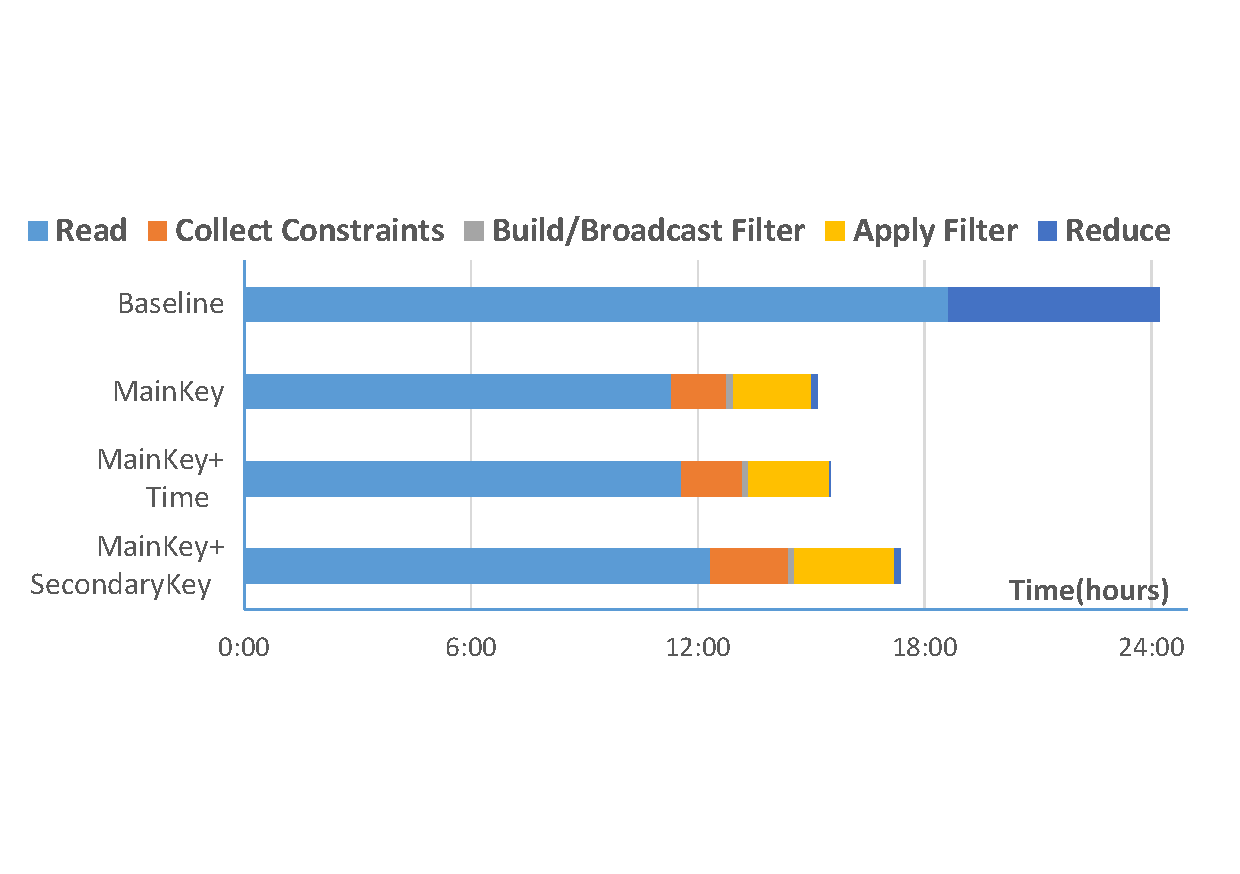
\includegraphics[clip, trim=0.5cm 3.5cm 0.9cm 3.5cm,
width=\columnwidth]{graphs_A5_breakdown.pdf}
\caption{A5}
\label{fig:A5}
\end{subfigure}
~
\begin{subfigure}[t]{\columnwidth}
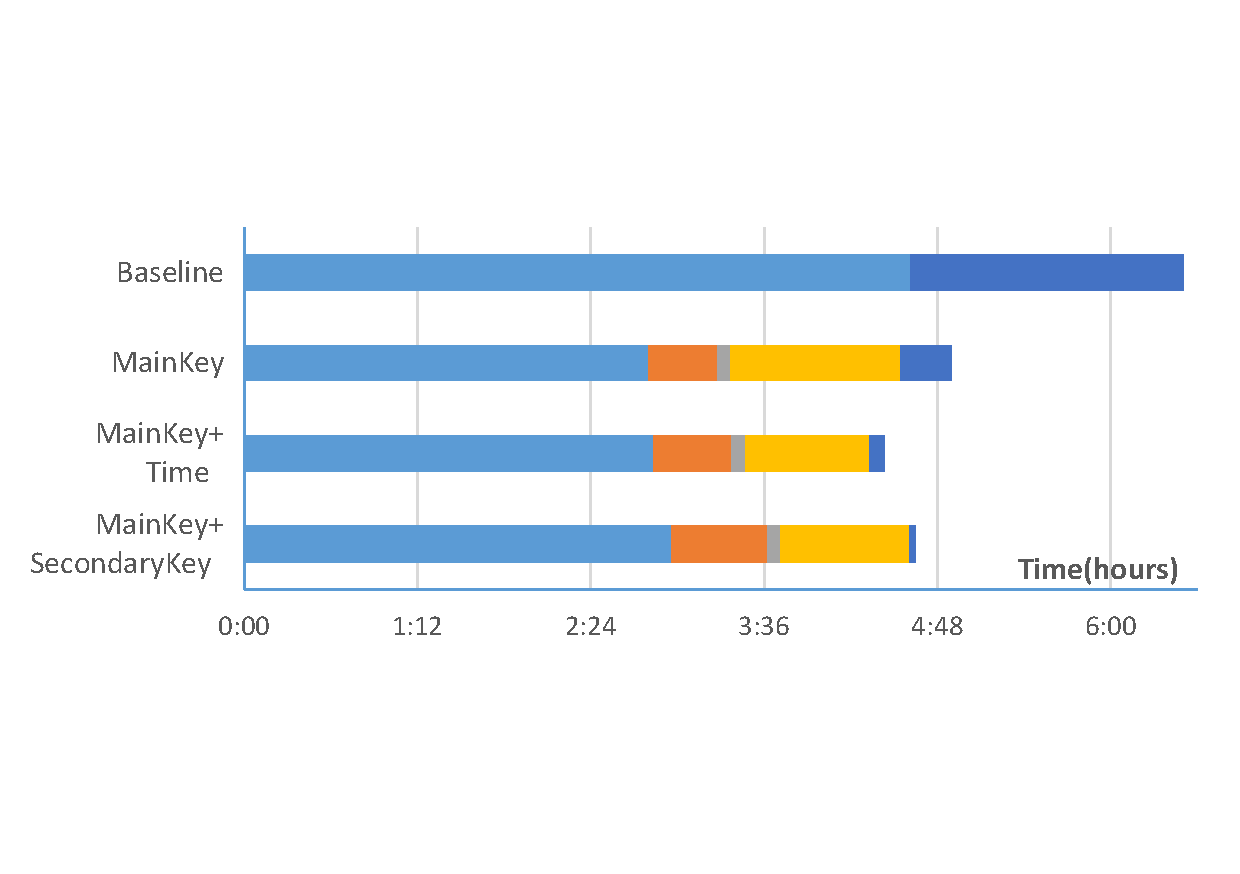
\includegraphics[clip, trim=0.5cm 4cm 0.9cm 4cm,
width=\columnwidth]{graphs_A3_breakdown.pdf}
\caption{A3}
\label{fig:A3}
\end{subfigure}

\caption{Breakdown of the total processing time for queries A5 and
A3.}
\label{fig:breakdown}
\end{figure}




\subsection{Latency speedup}


In terms of end-to-end running times we record speedups between 1.08x and 1.78x
for 8 out of the 18 queries in our workload, while for 4 of them our
approach performs within 5\% of the baseline (see Figure~\ref{fig:latency_red}).
Just like in the case of processing times, the slowdowns in latency mainly
correspond to queries for whom the abstract filters do not significantly reduce
the amount of data processed by the pattern matcher (below 5x).


We examine the performance of queries A12 and A13 as it highlights another
important factor in the latency speedup achieved by our approach.
While for both queries the abstract filters discard a significant number of the
input events and as such have smaller total processing times than the baseline,
only for A12 this translates in smaller end-to-end running times.
This happens due to the difference in the initial size of the input, 1.2TB for
A12 vs 307GB for A13, which when processed on a 85 nodes cluster results in
average running times of the reduction phase of 3.8 minutes for A12 vs 46
seconds for A13. 
Even though in our approach the reduction phase for A13 takes only 5.6 seconds
on average due to the smaller number of events being processed, that is not
enough to compensate for the additional latency introduced by the phases that
build and broadcast the abstract filters.
While the latency of these phases can be minimized by decentralizing the process
of building the abstract filters, developing and deploying such techniques falls 
outside the scope of our current work.
% same reason for A15


















\section{Conclusions and Future work}




\small
\bibliographystyle{abbrv}
\bibliography{main}




\end{document}
